
\section{First Models Comparison}
\label{part3}

\subsection{Testing protocol definition}


Each comparison is presented using as element of comparison the metric \textit{MSE}, as defined in section \ref{metrics}.
The models uses the default loss as defined in section \ref{loss}

The plot results are all presented with the same values of quantiles, the quantile $quantile(0.99)$ and the respective $quantile(0.01)$ but also the $quantile(0.9)$, $quantile(0.1)$ and the median.
Before the comparison between different models, we need to compare the impact of the values of the different hyperparameters of the problem.
The hyperparameters of the problem are :
\begin{itemize}
    \item The size of time series
    \item The learning rate of the model training
    \item The number of epochs of the training
    \item The output distribution, defined in section \ref{distribution}
    \item The individual hyperparameters of the different models
\end{itemize}
Each comparison section is interested in one particular hyperparameter of the problem.
In general the other hyperparameters takes default values, as given by GluonTS.

\subsection{Global Hyperparameters comparison}

\subsubsection{Different dataset configurations}

There is no quantitative comparison to do, considering that the goal is not to find the configuration which gives the better results. The quantitative results are not significant, except noticing that the results are indeed influenced by the configuration. 
In general the following section will consider configuration A as default, but if necessary other configuration will be tested.

\subsubsection{Time series size} \label{comp_lr}

\begin{figure}[H]
    \centering
    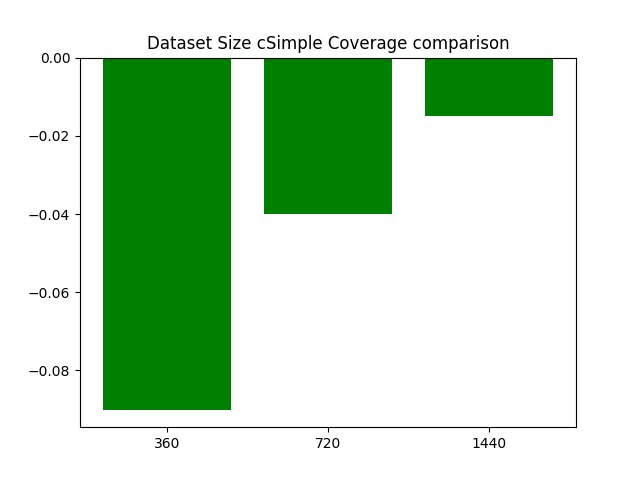
\includegraphics[width=300px]{plots/hist/a/datasize/cSimple/Coverage.png}
    %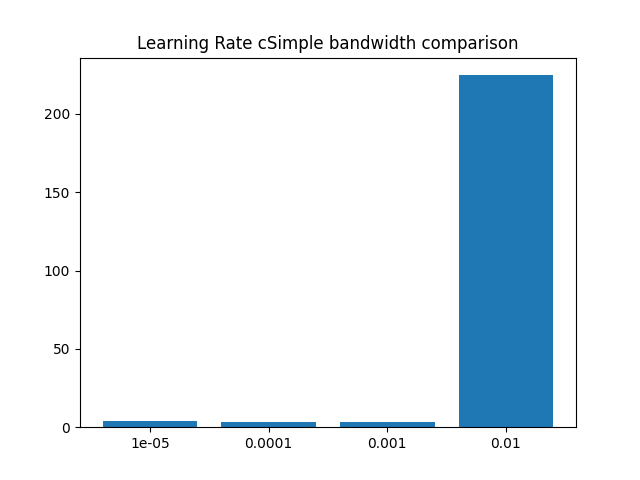
\includegraphics[width=200px]{plots/hist/a/lr/cSimple/bandwidth.png}
    %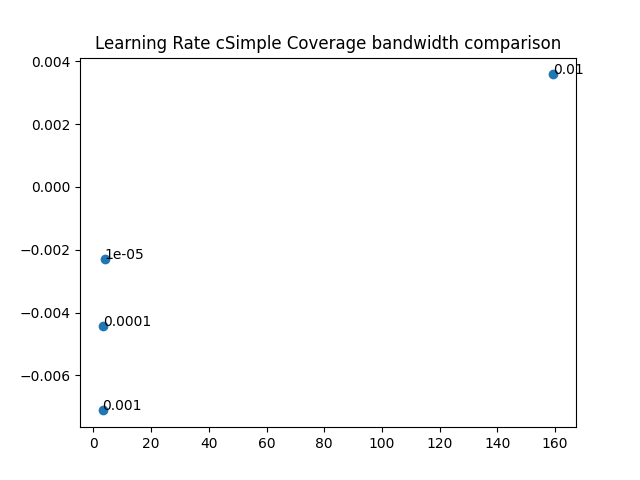
\includegraphics[width=300px]{plots/scatter/a/lr/cSimple/Coverage_bandwidth.png}
    \caption{Comparison of different time series size (Model: Simple (Default parameter values), Epochs = 100, $\alpha$ = 0.9, Distribution = Gaussian, Config A)}
    \label{fig:comp_datasize}
\end{figure}


\subsubsection{Learning rate} \label{comp_lr}

\begin{figure}[H]
    \centering
    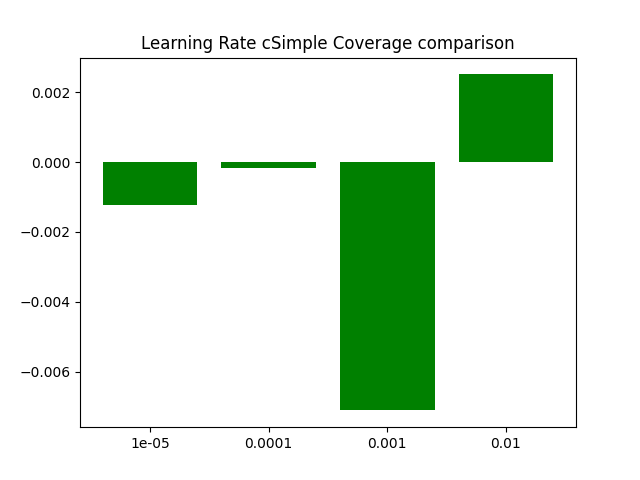
\includegraphics[width=300px]{plots/hist/a/lr/cSimple/Coverage.png}
    %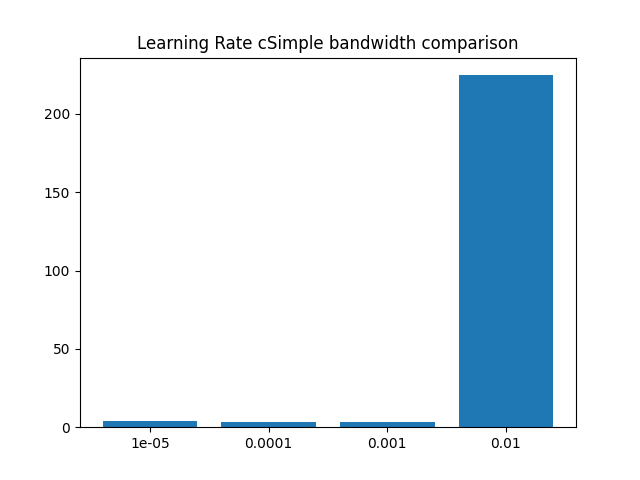
\includegraphics[width=200px]{plots/hist/a/lr/cSimple/bandwidth.png}
    %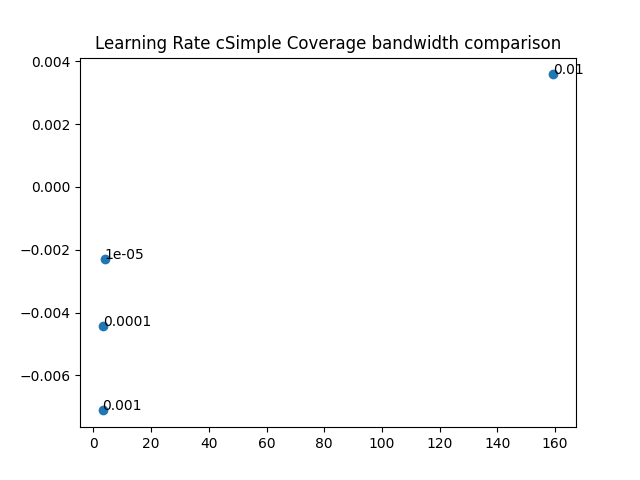
\includegraphics[width=300px]{plots/scatter/a/lr/cSimple/Coverage_bandwidth.png}
    \caption{Comparison of different learning rate (Model: Simple (Default parameter values), Epochs = 100, $\alpha$ = 0.9, Distribution = Gaussian, Config A)}
    \label{fig:comp_lr}
\end{figure}

The default learning rate in GluonTs for all deep learning models is $1^{-3}$
Learning rate as a great impact on the results.

\subsubsection{Epochs} \label{comp_epochs}

\begin{figure}[H]
    \centering
    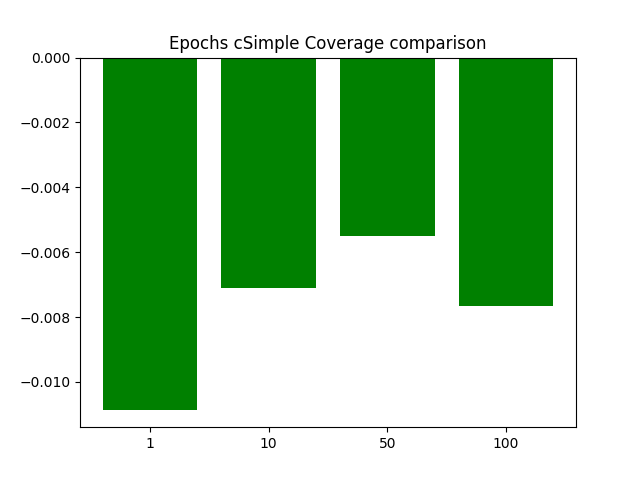
\includegraphics[width=300px]{plots/hist/a/epochs/cSimple/Coverage.png}
    %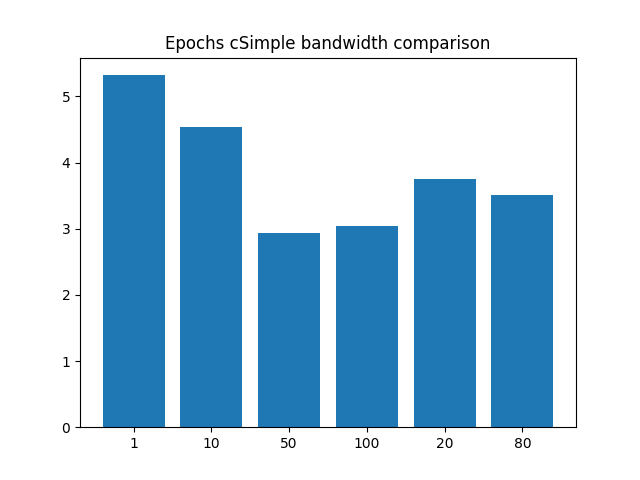
\includegraphics[width=200px]{plots/hist/a/epochs/cSimple/bandwidth.png}
    %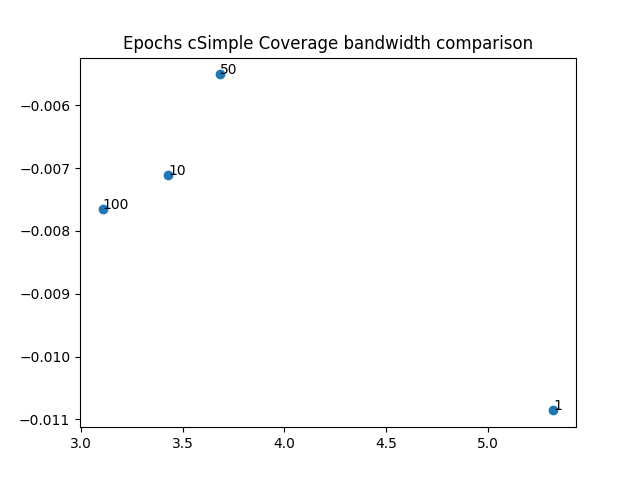
\includegraphics[width=300px]{plots/scatter/a/epochs/cSimple/Coverage_bandwidth.png}
    \caption{Comparison of different epochs number (Model: Simple (Default parameter values), $\alpha$ = 0.9, Distribution = Gaussian, Config A)}
    \label{fig:comp_epochs}
\end{figure}

All the deep learning models implemented must be trained a certain number of epochs. The default number 
is 100 epochs. This value is a good choice (better bandwidth of the comparison), as are values slightly  inferior (which have better Coverage). 

\newpage

\subsubsection{Output Distribution} \label{comp_outdistrib}

\begin{figure}[H]
    \centering
    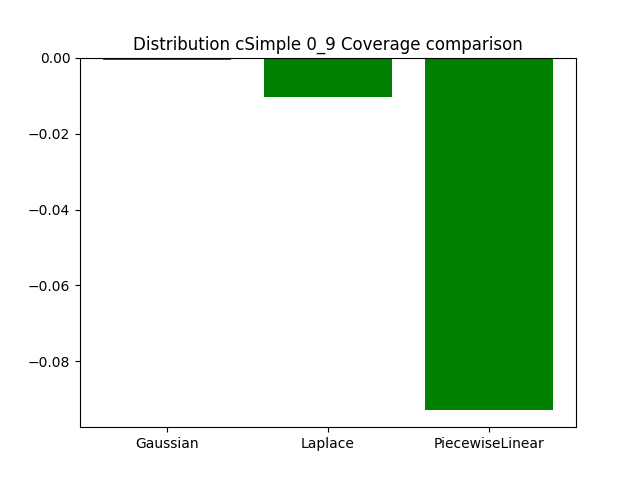
\includegraphics[width=300px]{plots/hist/a/distribution/cSimple/0_9/Coverage.png}
    %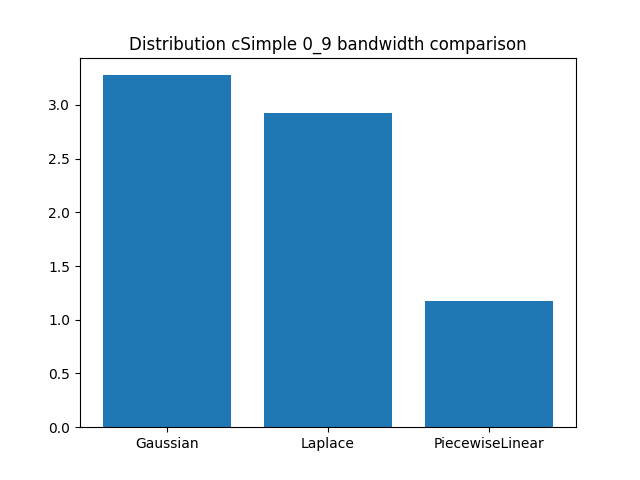
\includegraphics[width=200px]{plots/hist/a/distribution/cSimple/0_9/bandwidth.png}
    %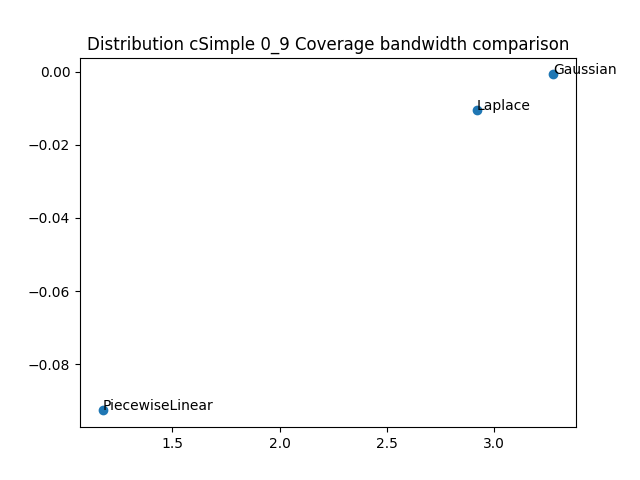
\includegraphics[width=300px]{plots/scatter/a/distribution/cSimple/0_9/Coverage_bandwidth.png}
    \caption{Comparison of different output distribution (Model: Simple (Default parameter values), Epochs = 100, $\alpha$ = 0.9,  Config A)}
    \label{fig:comp_outdistrib}
\end{figure}

% \textit{PiecewiseLinear} distribution gives very thin distribution but clearly underestimate the risk, and would be not chosen in consequence. Laplace gives slightly better results than Gaussian if we consider Coverage and bandwith as the same level of importance. 


\subsection{Different models parameters comparison and results} \label{comp_model_param}

The different models are described in the \ref{diff_models} section

\subsubsection{Simple} \label{comp_simple}

\begin{figure}[H]
    \centering
    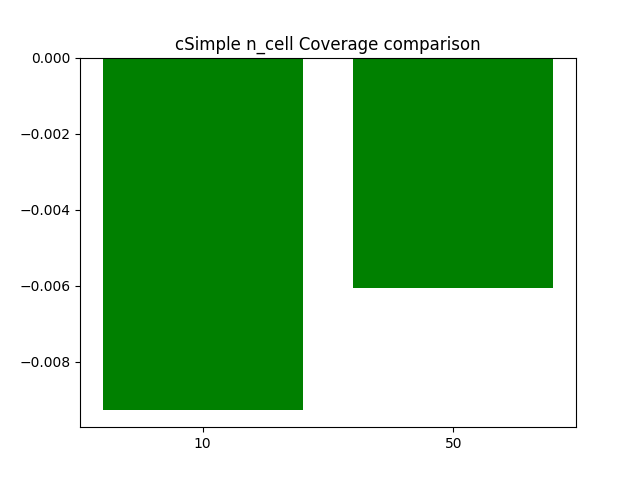
\includegraphics[width=300px]{plots/hist/a/cSimple/n_cell/Coverage.png}
    %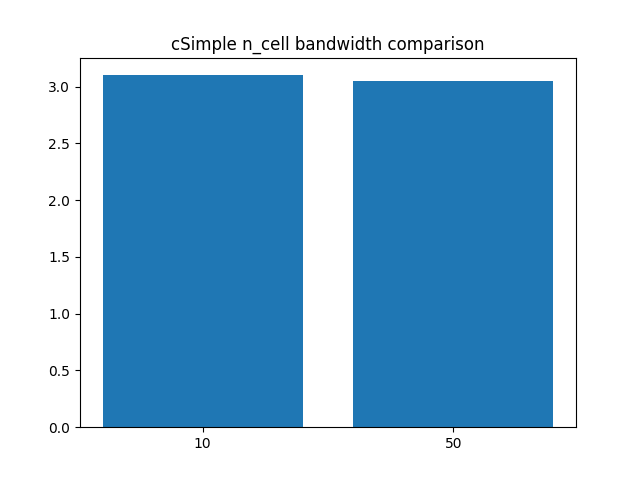
\includegraphics[width=200px]{plots/hist/a/cSimple/n_cell/bandwidth.png}
    %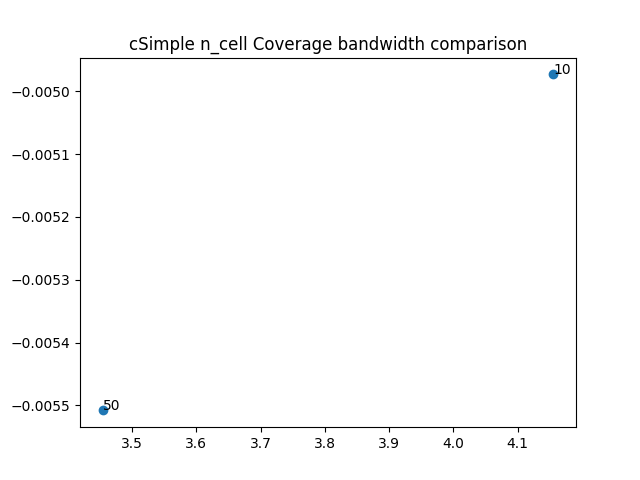
\includegraphics[width=300px]{plots/scatter/a/cSimple/n_cell/Coverage_bandwidth.png}
    \caption{Comparison of different $n\_cell$ values for Simple model (Epochs = 100, Distribution = Gaussian, $\alpha = 0.9$, Config A)}
    \label{fig:comp_simple}
\end{figure}

\begin{figure}[H]
    \centering
    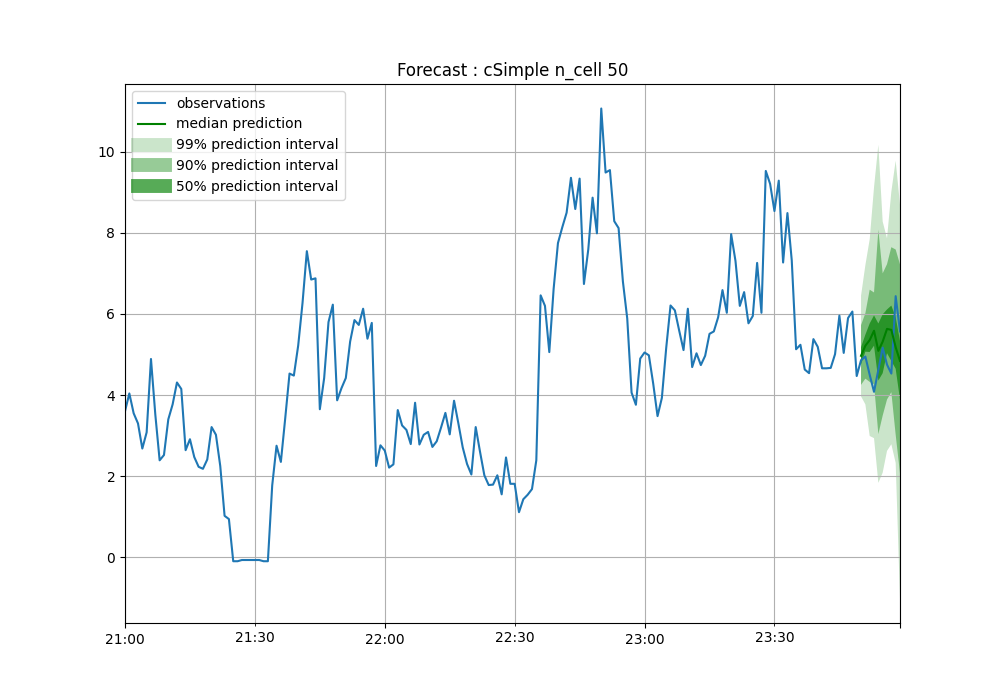
\includegraphics[width=400px]{plots/forecast/a/cSimple/n_cell/50/180.png}
    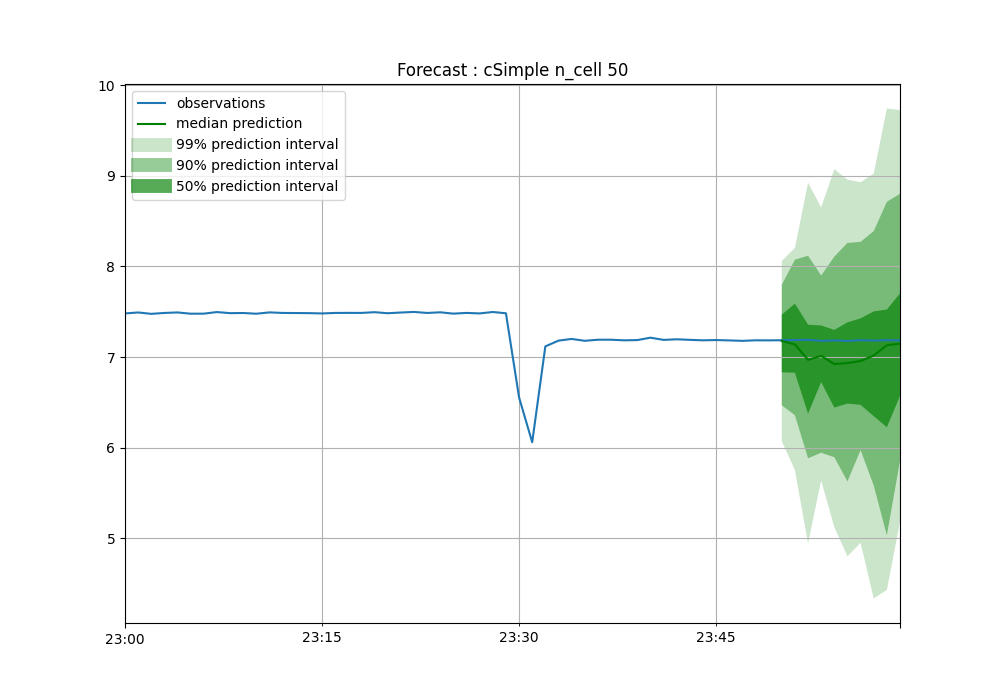
\includegraphics[width=400px]{plots/forecast/a/cSimple/n_cell/50/60.png}
    \caption{Forecast result of Simple model at 3 hours and 1 hour scale ($n\_cell = 50$ Epochs = 100, Distribution = Gaussian, $\alpha = 0.9$, Config A)}
    \label{fig:simple}
\end{figure}


\subsubsection{Simple Feed Fordward} \label{comp_feedfordward}

\begin{figure}[H]
    \centering
    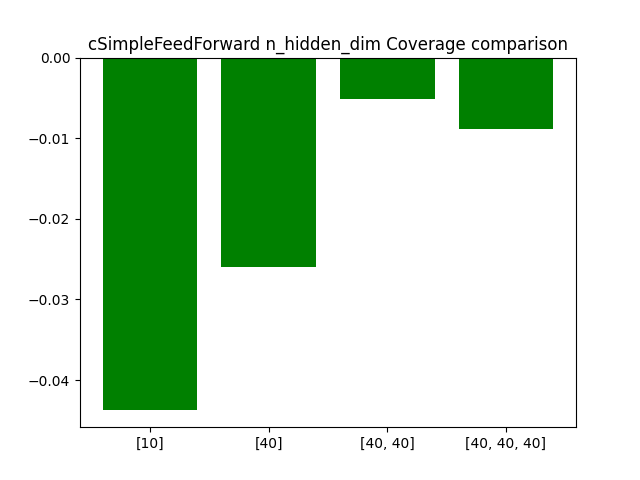
\includegraphics[width=300px]{plots/hist/a/cSimpleFeedForward/n_hidden_dim/Coverage.png}
    %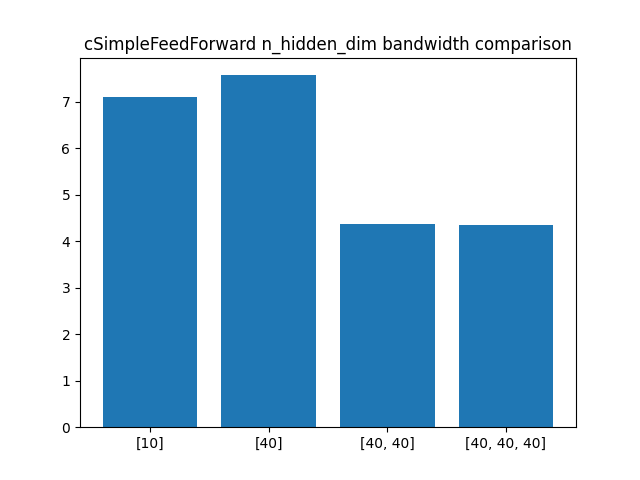
\includegraphics[width=200px]{plots/hist/a/cSimpleFeedForward/n_hidden_dim/bandwidth.png}
    %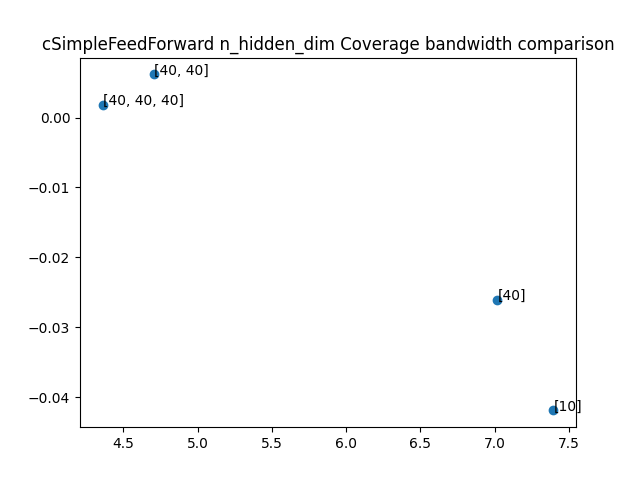
\includegraphics[width=300px]{plots/scatter/a/cSimpleFeedForward/n_hidden_dim/Coverage_bandwidth.png}
    \caption{Comparison of different $n\_hidden\_dim$ values for Simple FeedForward model (Epochs = 100, Distribution = Gaussian, $\alpha = 0.9$, Config A)}
    \label{fig:comp_feedfordward}
\end{figure}

\begin{figure}[H]
    \centering
    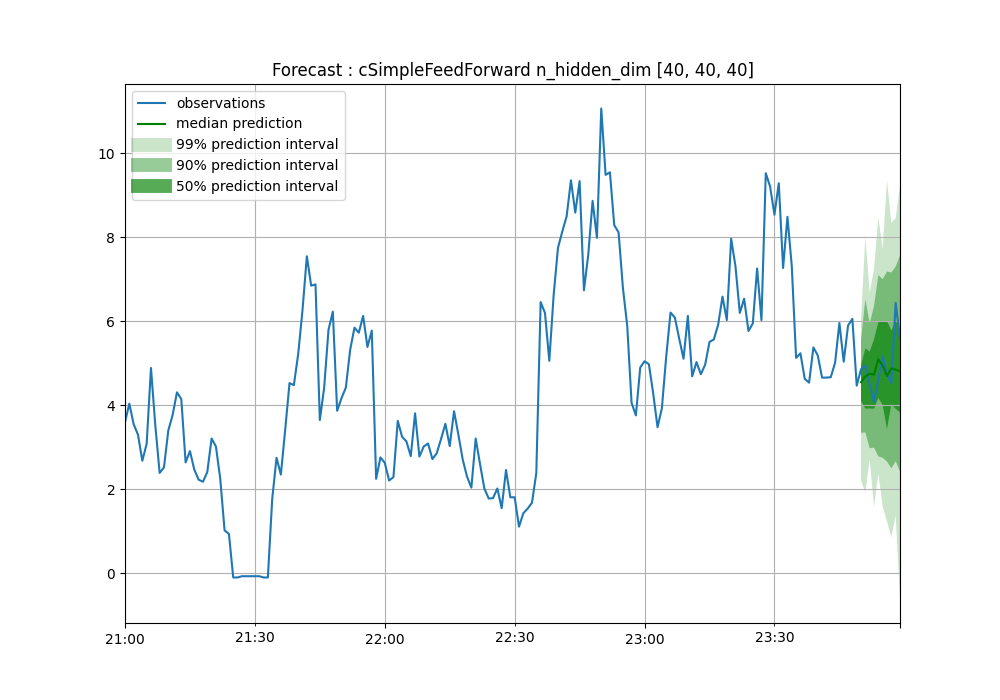
\includegraphics[width=400px]{plots/forecast/a/cSimpleFeedForward/n_hidden_dim/[40, 40, 40]/180.png}
    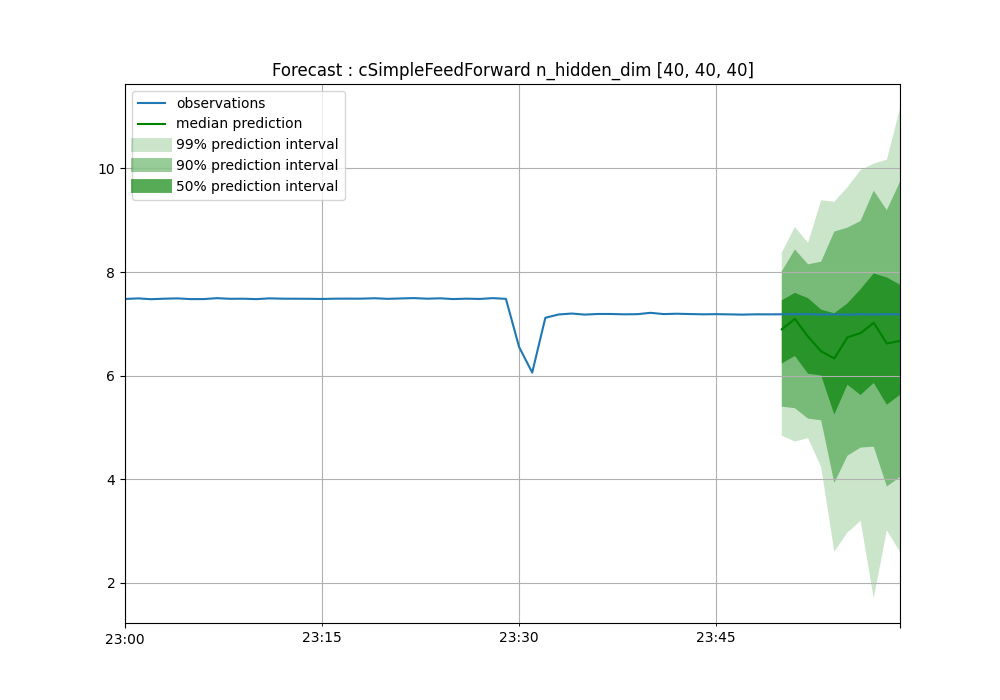
\includegraphics[width=400px]{plots/forecast/a/cSimpleFeedForward/n_hidden_dim/[40, 40, 40]/60.png}
    \caption{Forecast result of Simple FeedForward model at 3 hours and 1 hour scale ($n\_hidden_dim = [40,40,40]$ Epochs = 100, Distribution = Gaussian, $\alpha = 0.9$, Config A)}
    \label{fig:feedfordward}
\end{figure}


\subsubsection{Canonical RNN} \label{comp_canonicalrnn}

\begin{figure}[H]
    \centering
    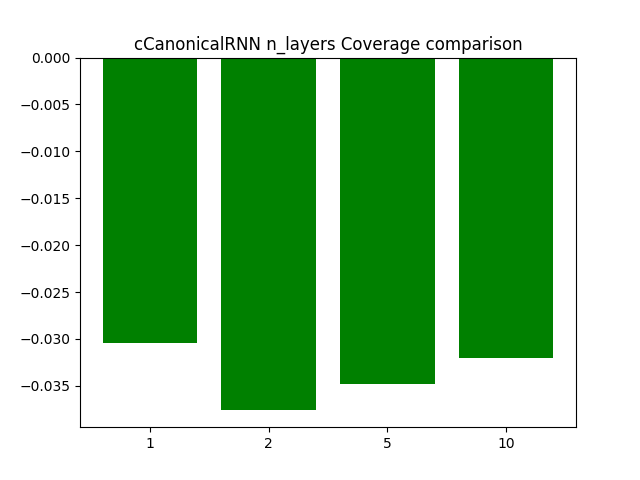
\includegraphics[width=300px]{plots/hist/a/cCanonicalRNN/n_layers/Coverage.png}
    %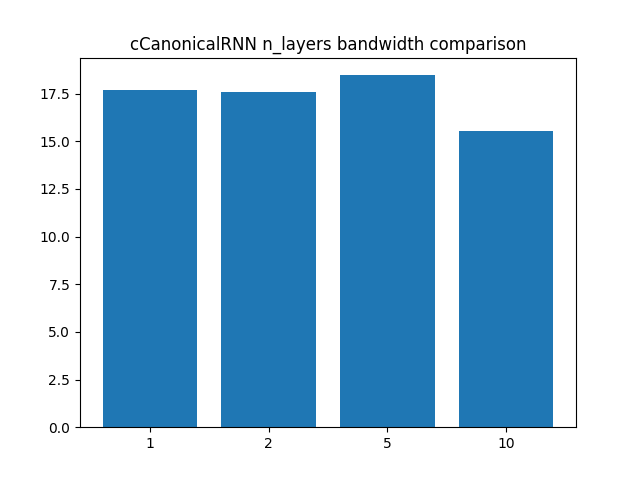
\includegraphics[width=200px]{plots/hist/a/cCanonicalRNN/n_layers/bandwidth.png}
    %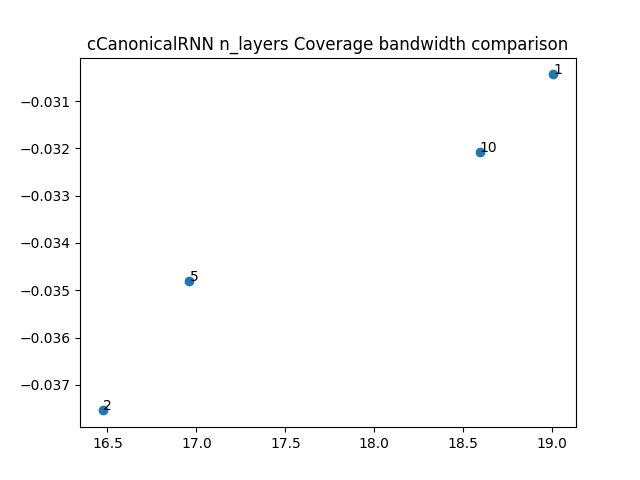
\includegraphics[width=300px]{plots/scatter/a/cCanonicalRNN/n_layers/Coverage_bandwidth.png}
    \caption{Comparison of different $n\_layers$ values for Canonical RNN model (Epochs = 100, Distribution = Gaussian, $\alpha = 0.9$, Config A)}
    \label{fig:comp_canonicalrnn}
\end{figure}

\begin{figure}[H]
    \centering
    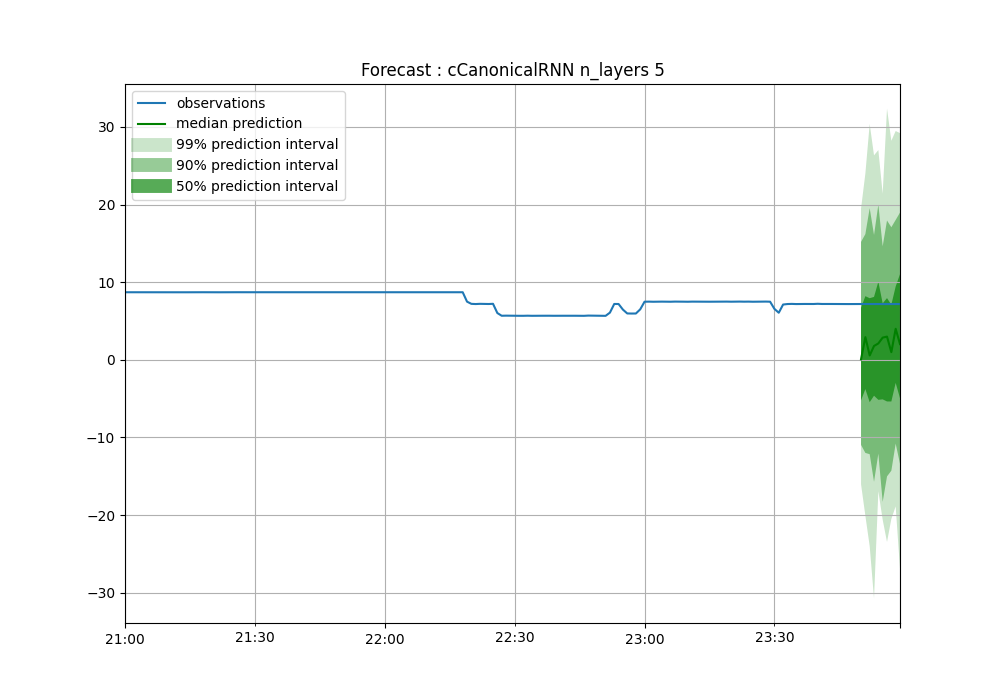
\includegraphics[width=400px]{plots/forecast/a/cCanonicalRNN/n_layers/5/180.png}
    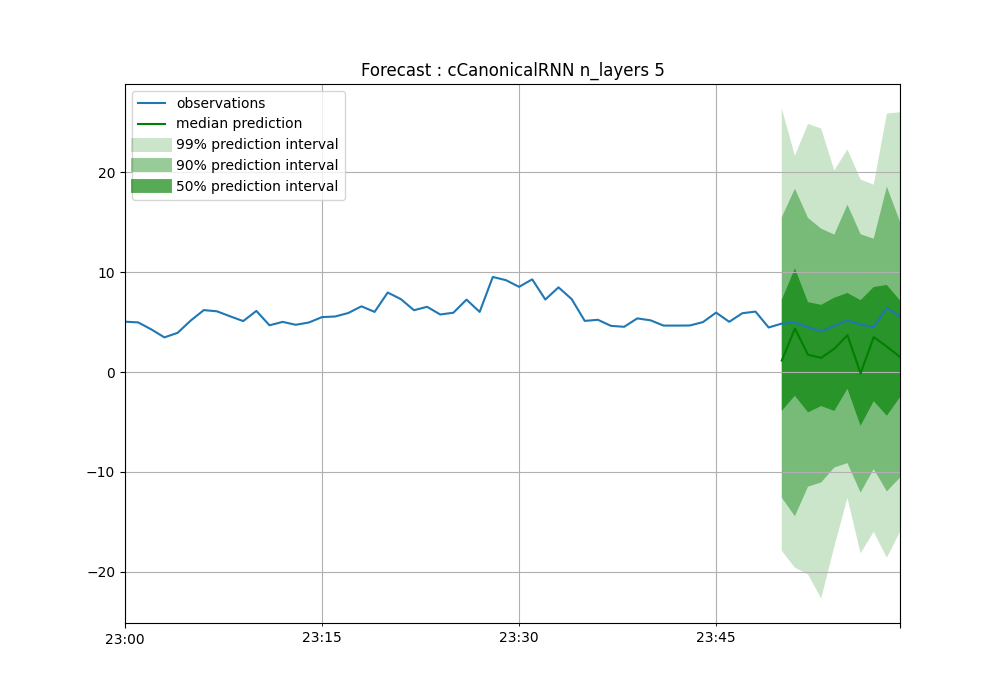
\includegraphics[width=400px]{plots/forecast/a/cCanonicalRNN/n_layers/5/60.png}
    \caption{Forecast result of Simple FeedForward model at 3 hours and 1 hour scale ($n\_layers = 5$ Epochs = 100, Distribution = Gaussian, $\alpha = 0.9$, Config A)}
    \label{fig:canonicalrnn}
\end{figure}


\subsubsection{Deep AR} \label{comp_deepar}

\begin{figure}[H]
    \centering
    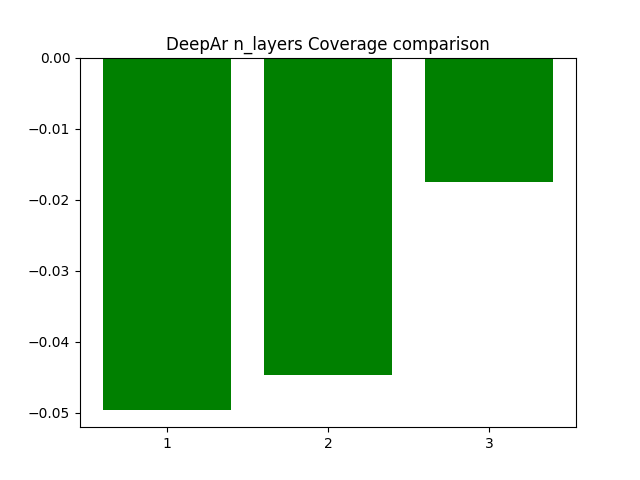
\includegraphics[width=300px]{plots/hist/a/DeepAr/n_layers/Coverage.png}
    %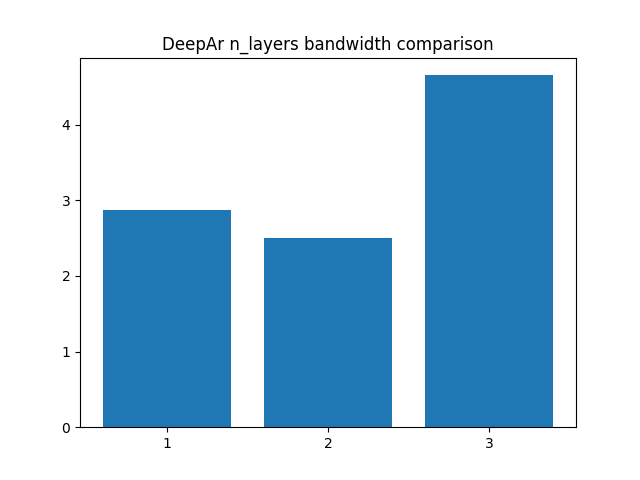
\includegraphics[width=200px]{plots/hist/a/DeepAr/n_layers/bandwidth.png}
    %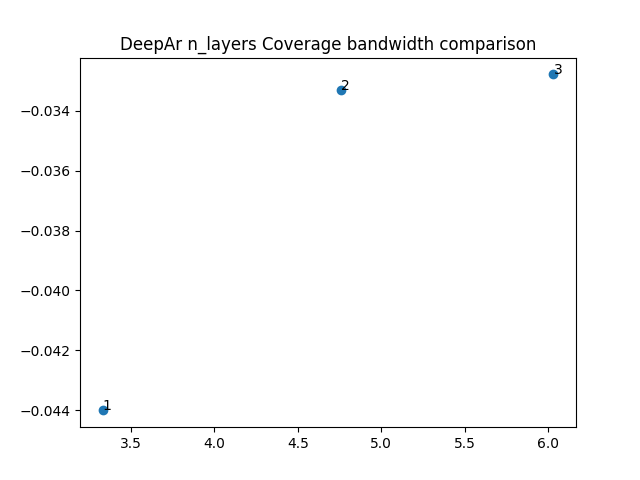
\includegraphics[width=300px]{plots/scatter/a/DeepAr/n_layers/Coverage_bandwidth.png}
    \caption{Comparison of different $n\_layers$ values for Deep AR model (Epochs = 100, Distribution = Gaussian, Config A)}
    \label{fig:comp_deepar_n_layers}
\end{figure}

\begin{figure}[H]
    \centering
    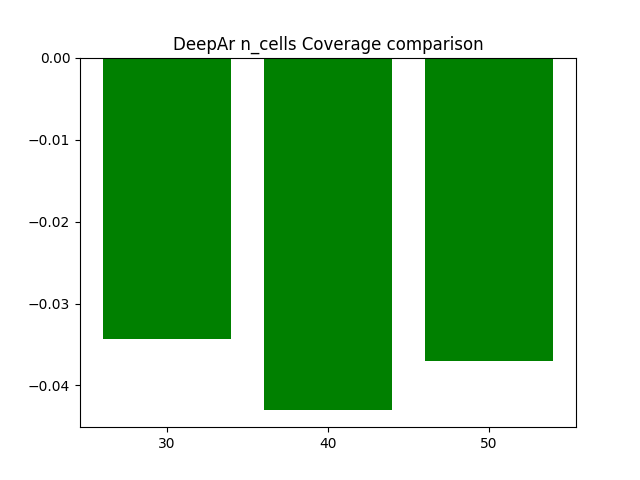
\includegraphics[width=300px]{plots/hist/a/DeepAr/n_cells/Coverage.png}
    %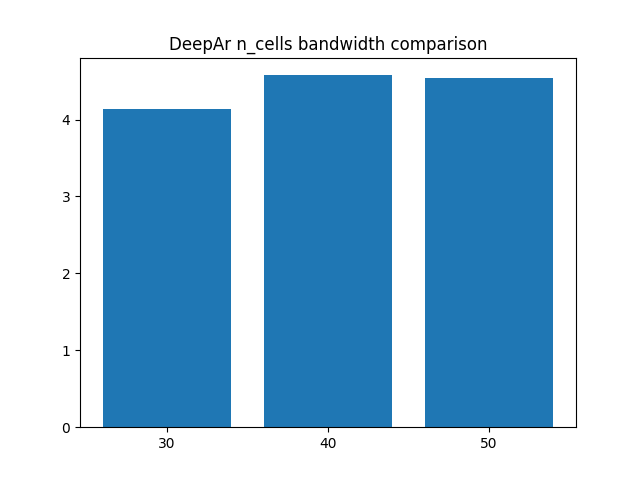
\includegraphics[width=200px]{plots/hist/a/DeepAr/n_cells/bandwidth.png}
    %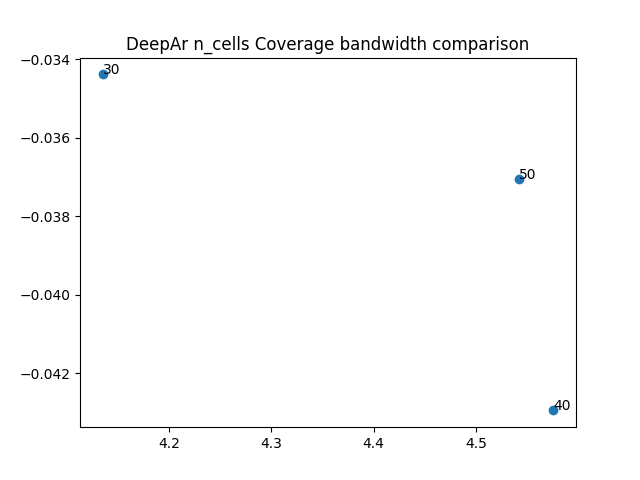
\includegraphics[width=300px]{plots/scatter/a/DeepAr/n_cells/Coverage_bandwidth.png}
    \caption{Comparison of different $n\_cells$ values for Deep AR model (Epochs = 100, Distribution = Gaussian, Config A)}
    \label{fig:comp_deepar_n_cells}
\end{figure}

\begin{figure}[H]
    \centering
    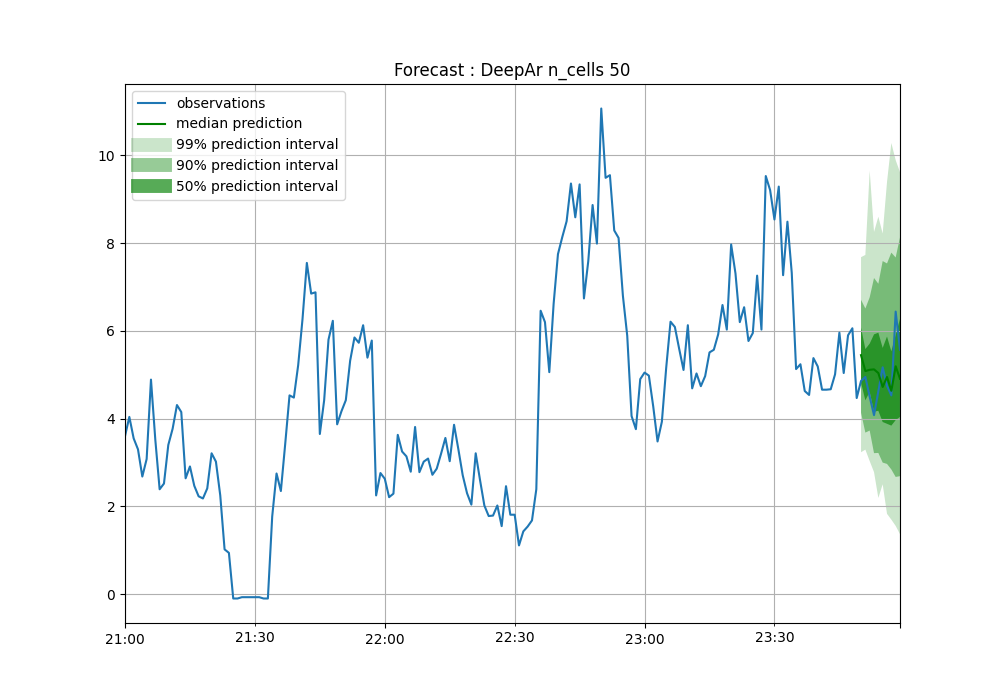
\includegraphics[width=400px]{plots/forecast/a/DeepAr/n_cells/50/180.png}
    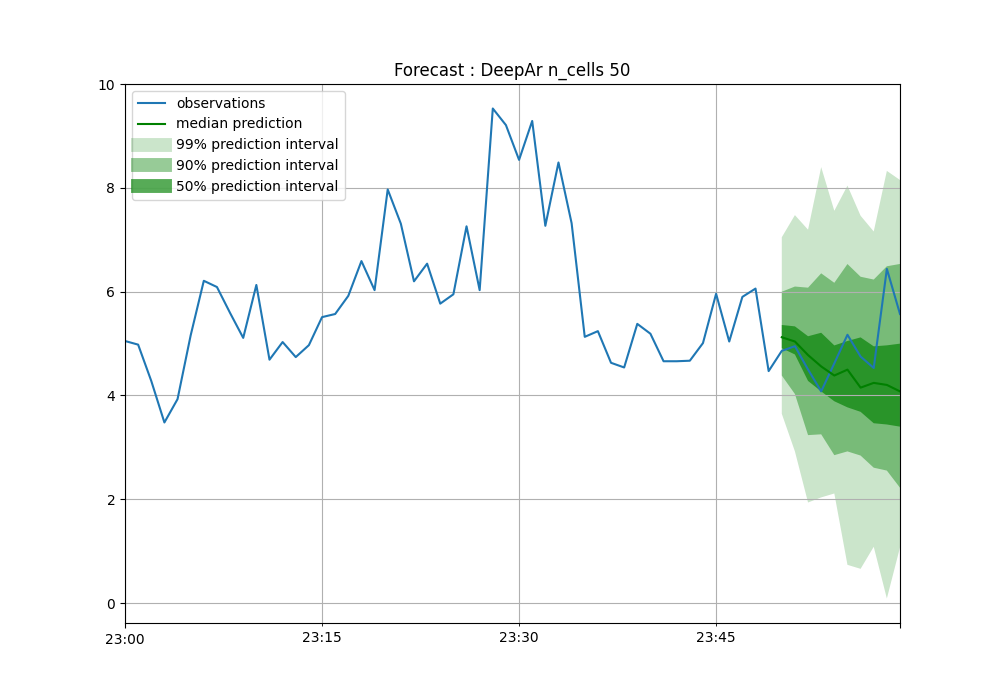
\includegraphics[width=400px]{plots/forecast/a/DeepAr/n_cells/50/60.png}
    \caption{Forecast result of Deep Ar model at 3 hours and 1 hour scale ($n\_layers = 2$, $n\_cells = 50$, Epochs = 100, Distribution = Gaussian, Config A)}
    \label{fig:deepar}
\end{figure}

\subsubsection{Deep Factor} \label{comp_deepfactor}

\begin{figure}[H]
    \centering
    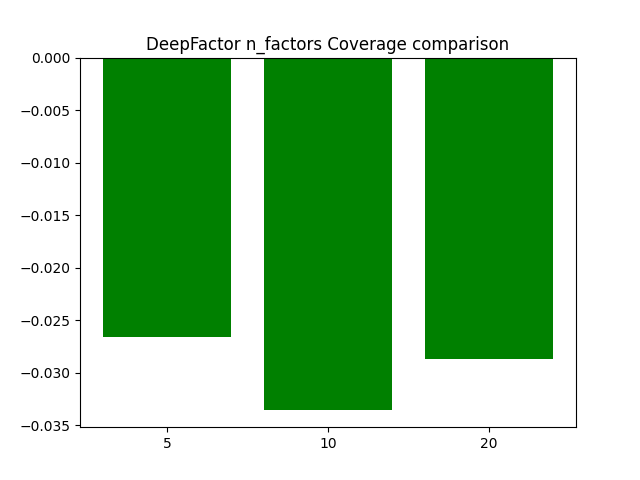
\includegraphics[width=300px]{plots/hist/a/DeepFactor/n_factors/Coverage.png}
    %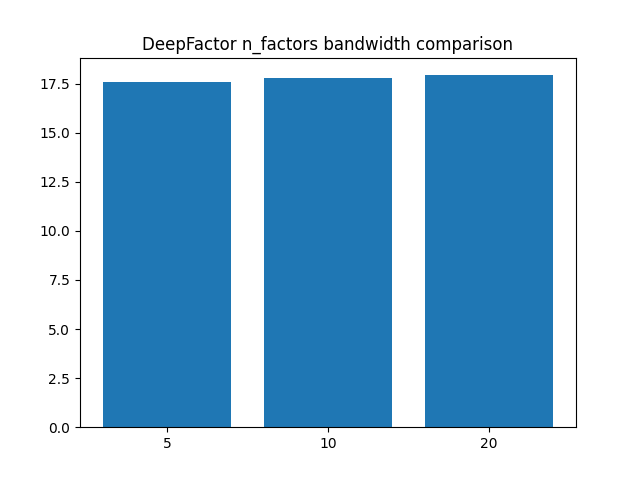
\includegraphics[width=200px]{plots/hist/a/DeepFactor/n_factors/bandwidth.png}
    %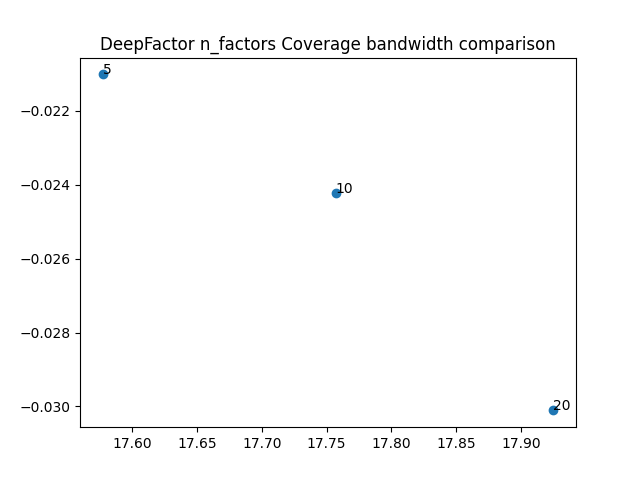
\includegraphics[width=300px]{plots/scatter/a/DeepFactor/n_factors/Coverage_bandwidth.png}
    \caption{Comparison of different $n\_factors$ values for Deep Factors model (Epochs = 100, Distribution = Gaussian, $\alpha = 0.9$, Config A)}
    \label{fig:comp_deepfactor_n_factors}
\end{figure}

\begin{figure}[H]
    \centering
    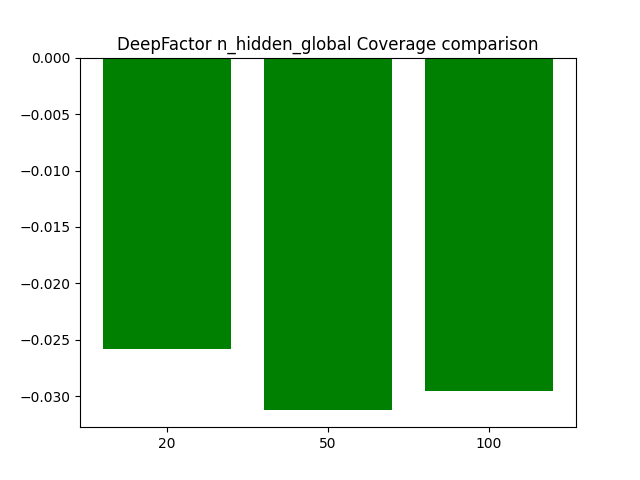
\includegraphics[width=300px]{plots/hist/a/DeepFactor/n_hidden_global/Coverage.png}
    %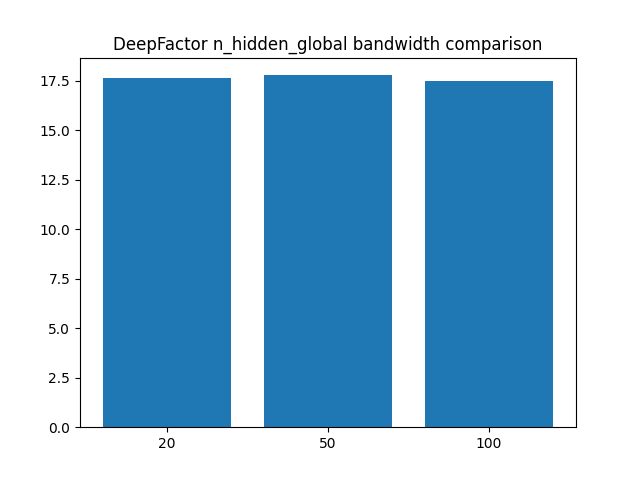
\includegraphics[width=200px]{plots/hist/a/DeepFactor/n_hidden_global/bandwidth.png}
    %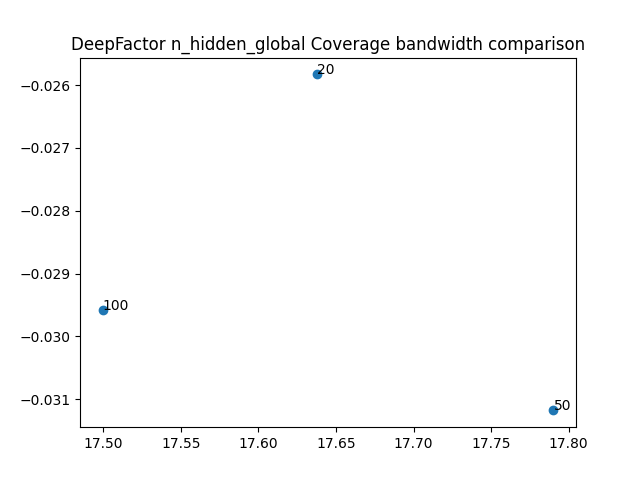
\includegraphics[width=300px]{plots/scatter/a/DeepFactor/n_hidden_global/Coverage_bandwidth.png}
    \caption{Comparison of different $n\_hidden\_global$ values for Deep Factors model (Epochs = 100, Distribution = Gaussian, $\alpha = 0.9$, Config A)}
    \label{fig:comp_deepfactor_n_hidden_globals}
\end{figure}

\begin{figure}[H]
    \centering
    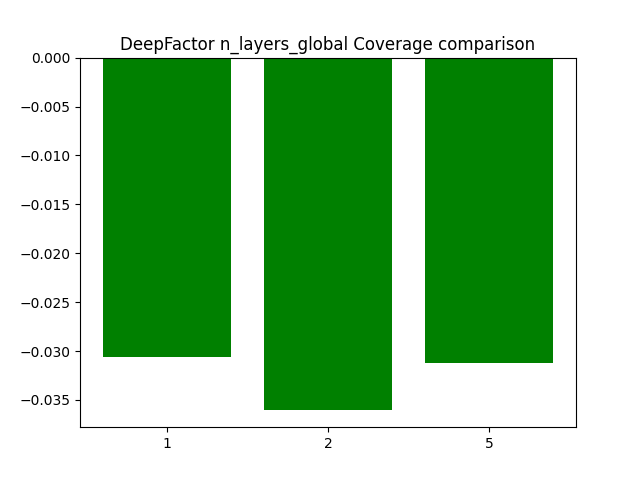
\includegraphics[width=300px]{plots/hist/a/DeepFactor/n_layers_global/Coverage.png}
    %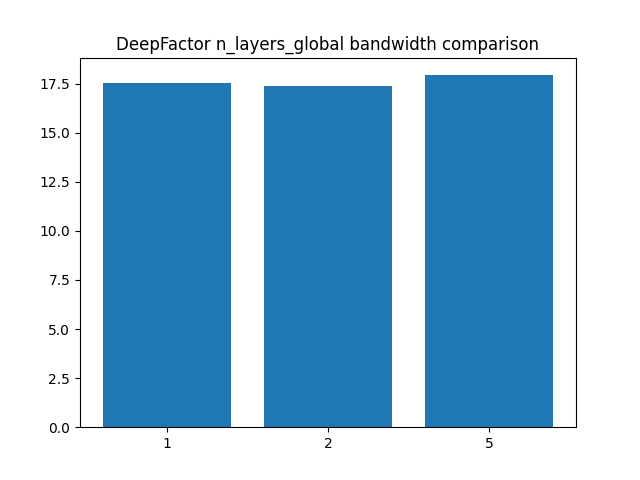
\includegraphics[width=200px]{plots/hist/a/DeepFactor/n_layers_global/bandwidth.png}
    %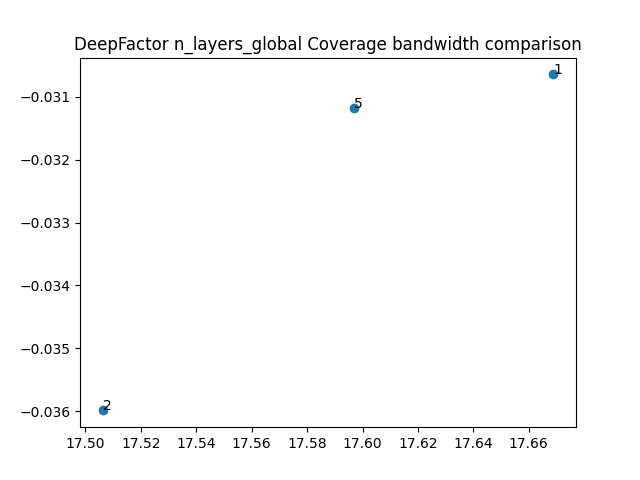
\includegraphics[width=300px]{plots/scatter/a/DeepFactor/n_layers_global/Coverage_bandwidth.png}
    \caption{Comparison of different $n\_layers\_global$ values for Deep Factors model (Epochs = 100, Distribution = Gaussian, $\alpha = 0.9$, Config A)}
    \label{fig:comp_deepfactor_n_layers_global}
\end{figure}

\begin{figure}[H]
    \centering
    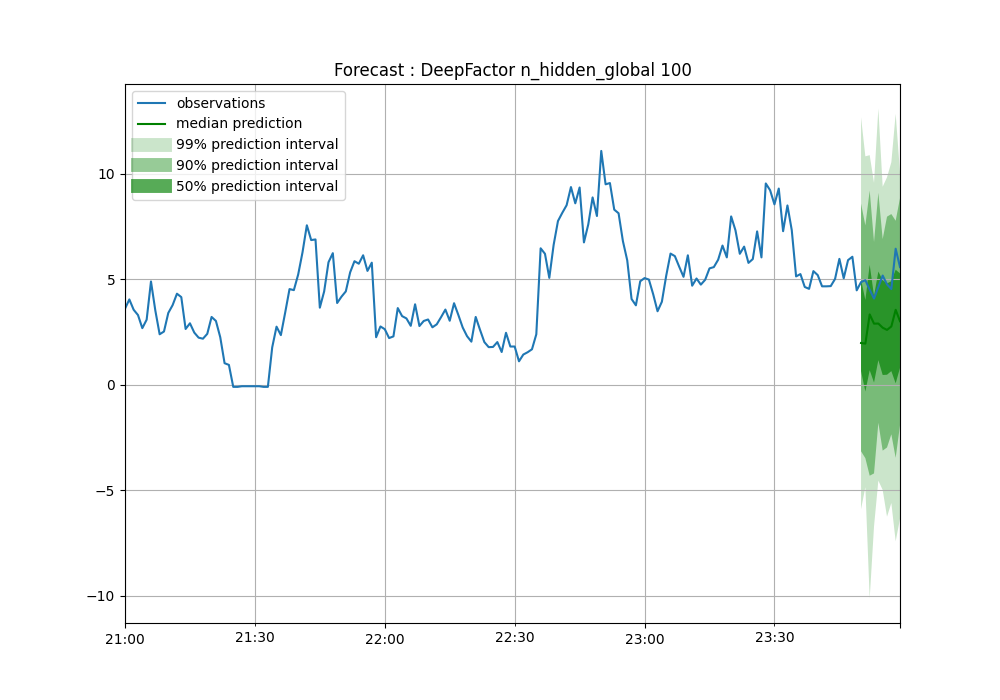
\includegraphics[width=400px]{plots/forecast/a/DeepFactor/n_hidden_global/100/180.png}
    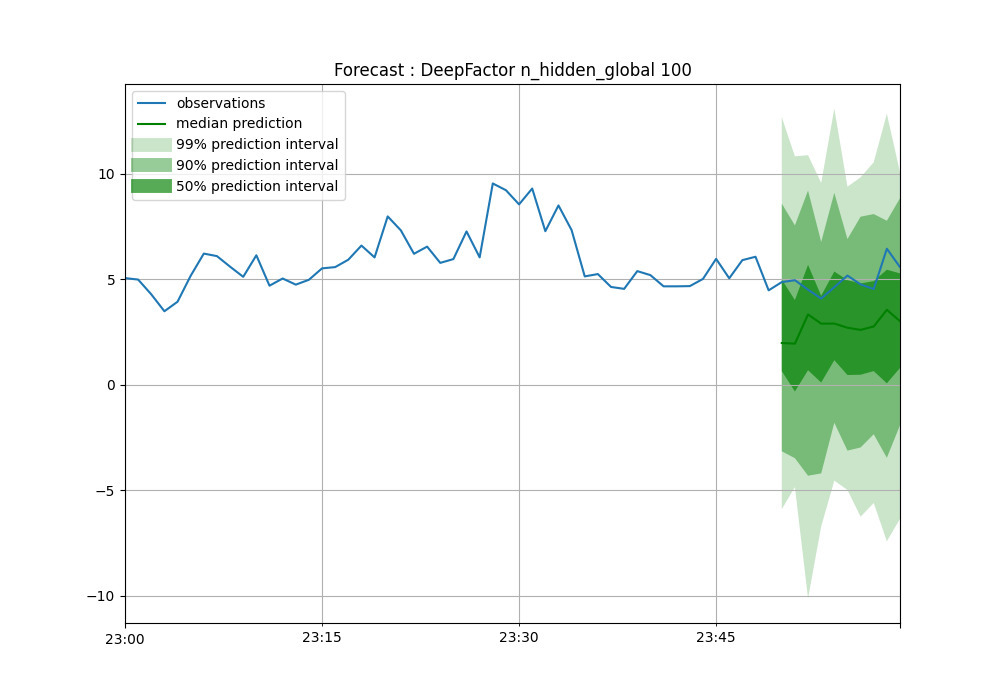
\includegraphics[width=400px]{plots/forecast/a/DeepFactor/n_hidden_global/100/60.png}
    \caption{Forecast result of Deep Factors model at 3 hours and 1 hour scale ($n\_factors = 5$, $n\_hidden\_global = 100$, $n\_layers\_global = 1$ Epochs = 100, Distribution = Gaussian, $\alpha = 0.9$, Config A)}
    \label{fig:comp_deepfactor_n_hidden_global}
\end{figure}

Contrary to another model, different hyperparameters of Deep Factors had a relatively low impact on the quality of the model.

\subsubsection{MQCNN} \label{comp_mqcnn}

\begin{figure}[H]
    \centering
    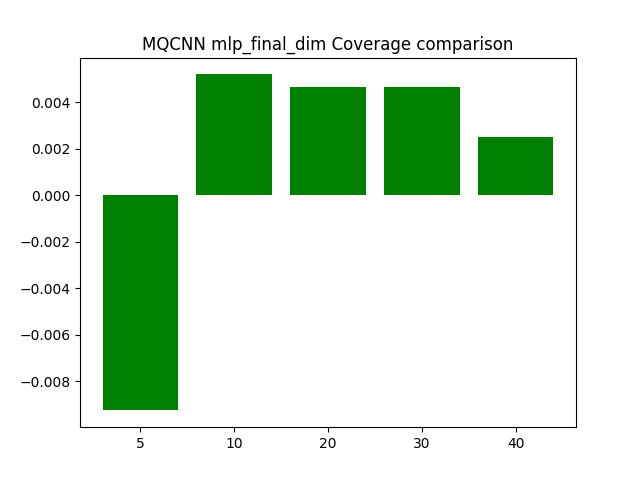
\includegraphics[width=300px]{plots/hist/a/MQCNN/mlp_final_dim/Coverage.png}
    %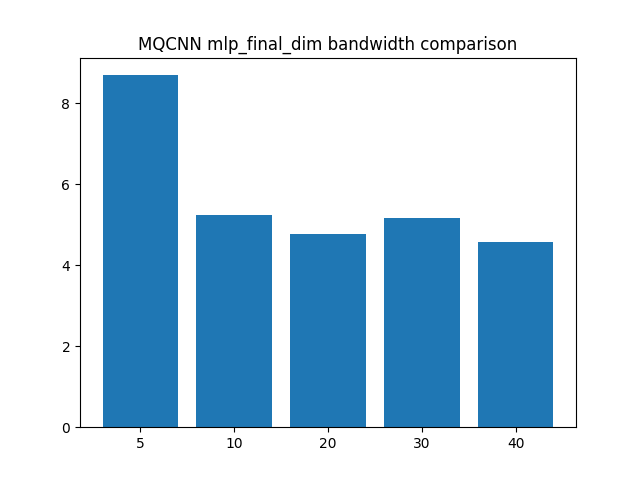
\includegraphics[width=200px]{plots/hist/a/MQCNN/mlp_final_dim/bandwidth.png}
    %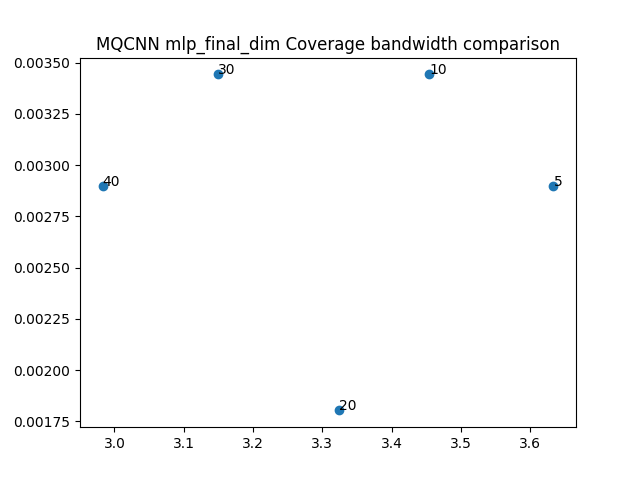
\includegraphics[width=300px]{plots/scatter/a/MQCNN/mlp_final_dim/Coverage_bandwidth.png}
    \caption{Comparison of different $mlp\_final\_dim$ values for MQCNN model (Epochs = 100, Distribution = Gaussian, Config A)}
    \label{fig:comp_mqcnn}
\end{figure}

\begin{figure}[H]
    \centering
    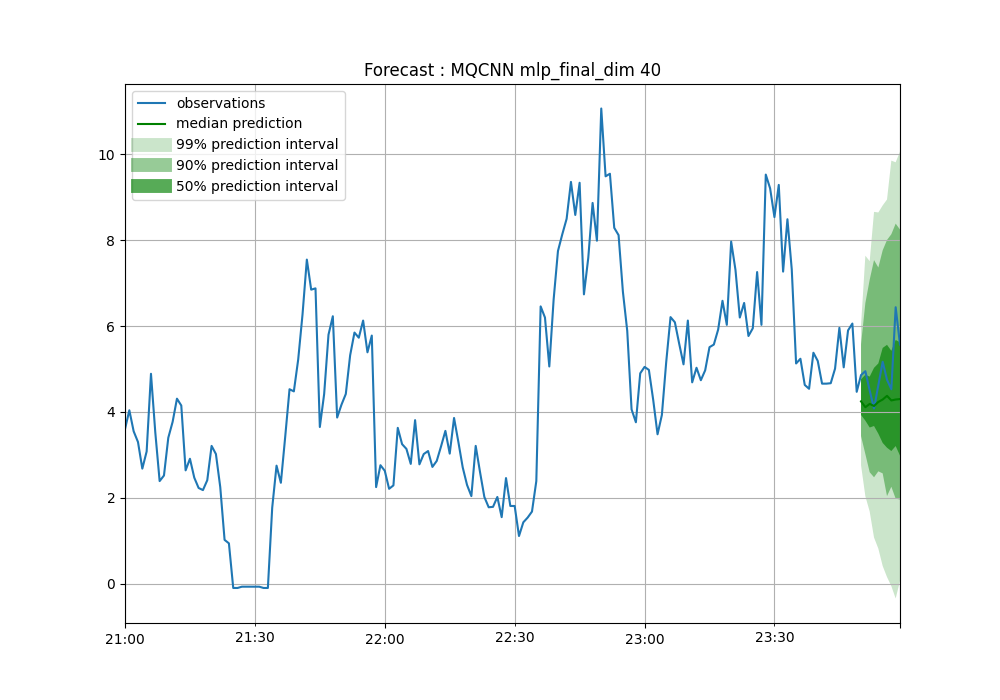
\includegraphics[width=400px]{plots/forecast/a/MQCNN/mlp_final_dim/40/180.png}
    \includegraphics[width=400px]{plots/forecast/a/MQCNN/mlp_final_dim/40/60.png}
    \caption{Forecast result of MQCNN model at 3 hours and 1 hour scale ($mlp\_final\_dim = 40 $, Epochs = 100, Distribution = Gaussian, Config A)}
    \label{fig:mqcnn}
\end{figure}

\subsubsection{MQRNN} \label{comp_mqrnn}

\begin{figure}[H]
    \centering
    \includegraphics[width=300px]{plots/hist/a/MQRNN/mlp_final_dim/Coverage.png}
    %\includegraphics[width=200px]{plots/hist/a/MQRNN/mlp_final_dim/bandwidth.png}
    %\includegraphics[width=300px]{plots/scatter/a/MQRNN/mlp_final_dim/Coverage_bandwidth.png}
    \caption{Comparison of different $mlp\_final\_dim$ values for MQRNN model (Epochs = 100, Distribution = Gaussian, Config A)}
    \label{fig:comp_mqrnn}
\end{figure}

\begin{figure}[H]
    \centering
    \includegraphics[width=400px]{plots/forecast/a/MQRNN/mlp_final_dim/20/180.png}
    \includegraphics[width=400px]{plots/forecast/a/MQRNN/mlp_final_dim/20/60.png}
    \caption{Forecast result of MQRNN model at 3 hours and 1 hour scale ($mlp\_final\_dim = 20 $, Epochs = 100, Distribution = Gaussian, Config A)}
    \label{fig:mqrnn}
\end{figure}


\subsubsection{Gaussian Process} \label{comp_gp}

\begin{figure}[H]
    \centering
    \includegraphics[width=400px]{plots/forecast/a/model/Gaussian/0_9/GaussianProcess/180.png}
    \includegraphics[width=400px]{plots/forecast/a/model/Gaussian/0_9/GaussianProcess/60.png}
    \caption{Forecast result of Gaussian Process model at 3 hours and 1 hour scale (, Epochs = 100, Distribution = Gaussian, Config A)}
    \label{fig:gp}
\end{figure}


\subsubsection{NPTS} \label{comp_npts}

\begin{figure}[H]
    \centering
    \includegraphics[width=400px]{plots/forecast/a/model/Gaussian/0_9/NPTS/180.png}
    \includegraphics[width=400px]{plots/forecast/a/model/Gaussian/0_9/NPTS/60.png}
    \caption{Forecast result of NPTS model at 3 hours and 1 hour scale (Epochs = 100, Config A)}
    \label{fig:npts}
\end{figure}

\subsubsection{ETS} \label{comp_ets}

\begin{figure}[H]
    \centering
    \includegraphics[width=400px]{plots/forecast/a/model/Gaussian/0_9/NPTS/180.png}
    \includegraphics[width=400px]{plots/forecast/a/model/Gaussian/0_9/NPTS/60.png}
    \caption{Forecast result of ETS model at 3 hours and 1 hour scale (Epochs = 100, Config A)}
    \label{fig:ets}
\end{figure}

\subsection{Global comparison}

\begin{figure}[H]
    \centering
    \includegraphics[width=200px]{plots/hist/a/model/0_9/Gaussian/Coverage.png}
    %\includegraphics[width=200px]{plots/hist/a/model/0_9/Gaussian/bandwidth.png}
    %\includegraphics[width=300px]{plots/scatter/a/model/0_9/Gaussian/Coverage_bandwidth.png}
    \caption{Comparison of different models (Epochs = 100, Distribution = Gaussian, Config A)}
    \label{fig:comp_mqcnn}
\end{figure}

